\section{Bilder}

\begin{figure}
    \centering
    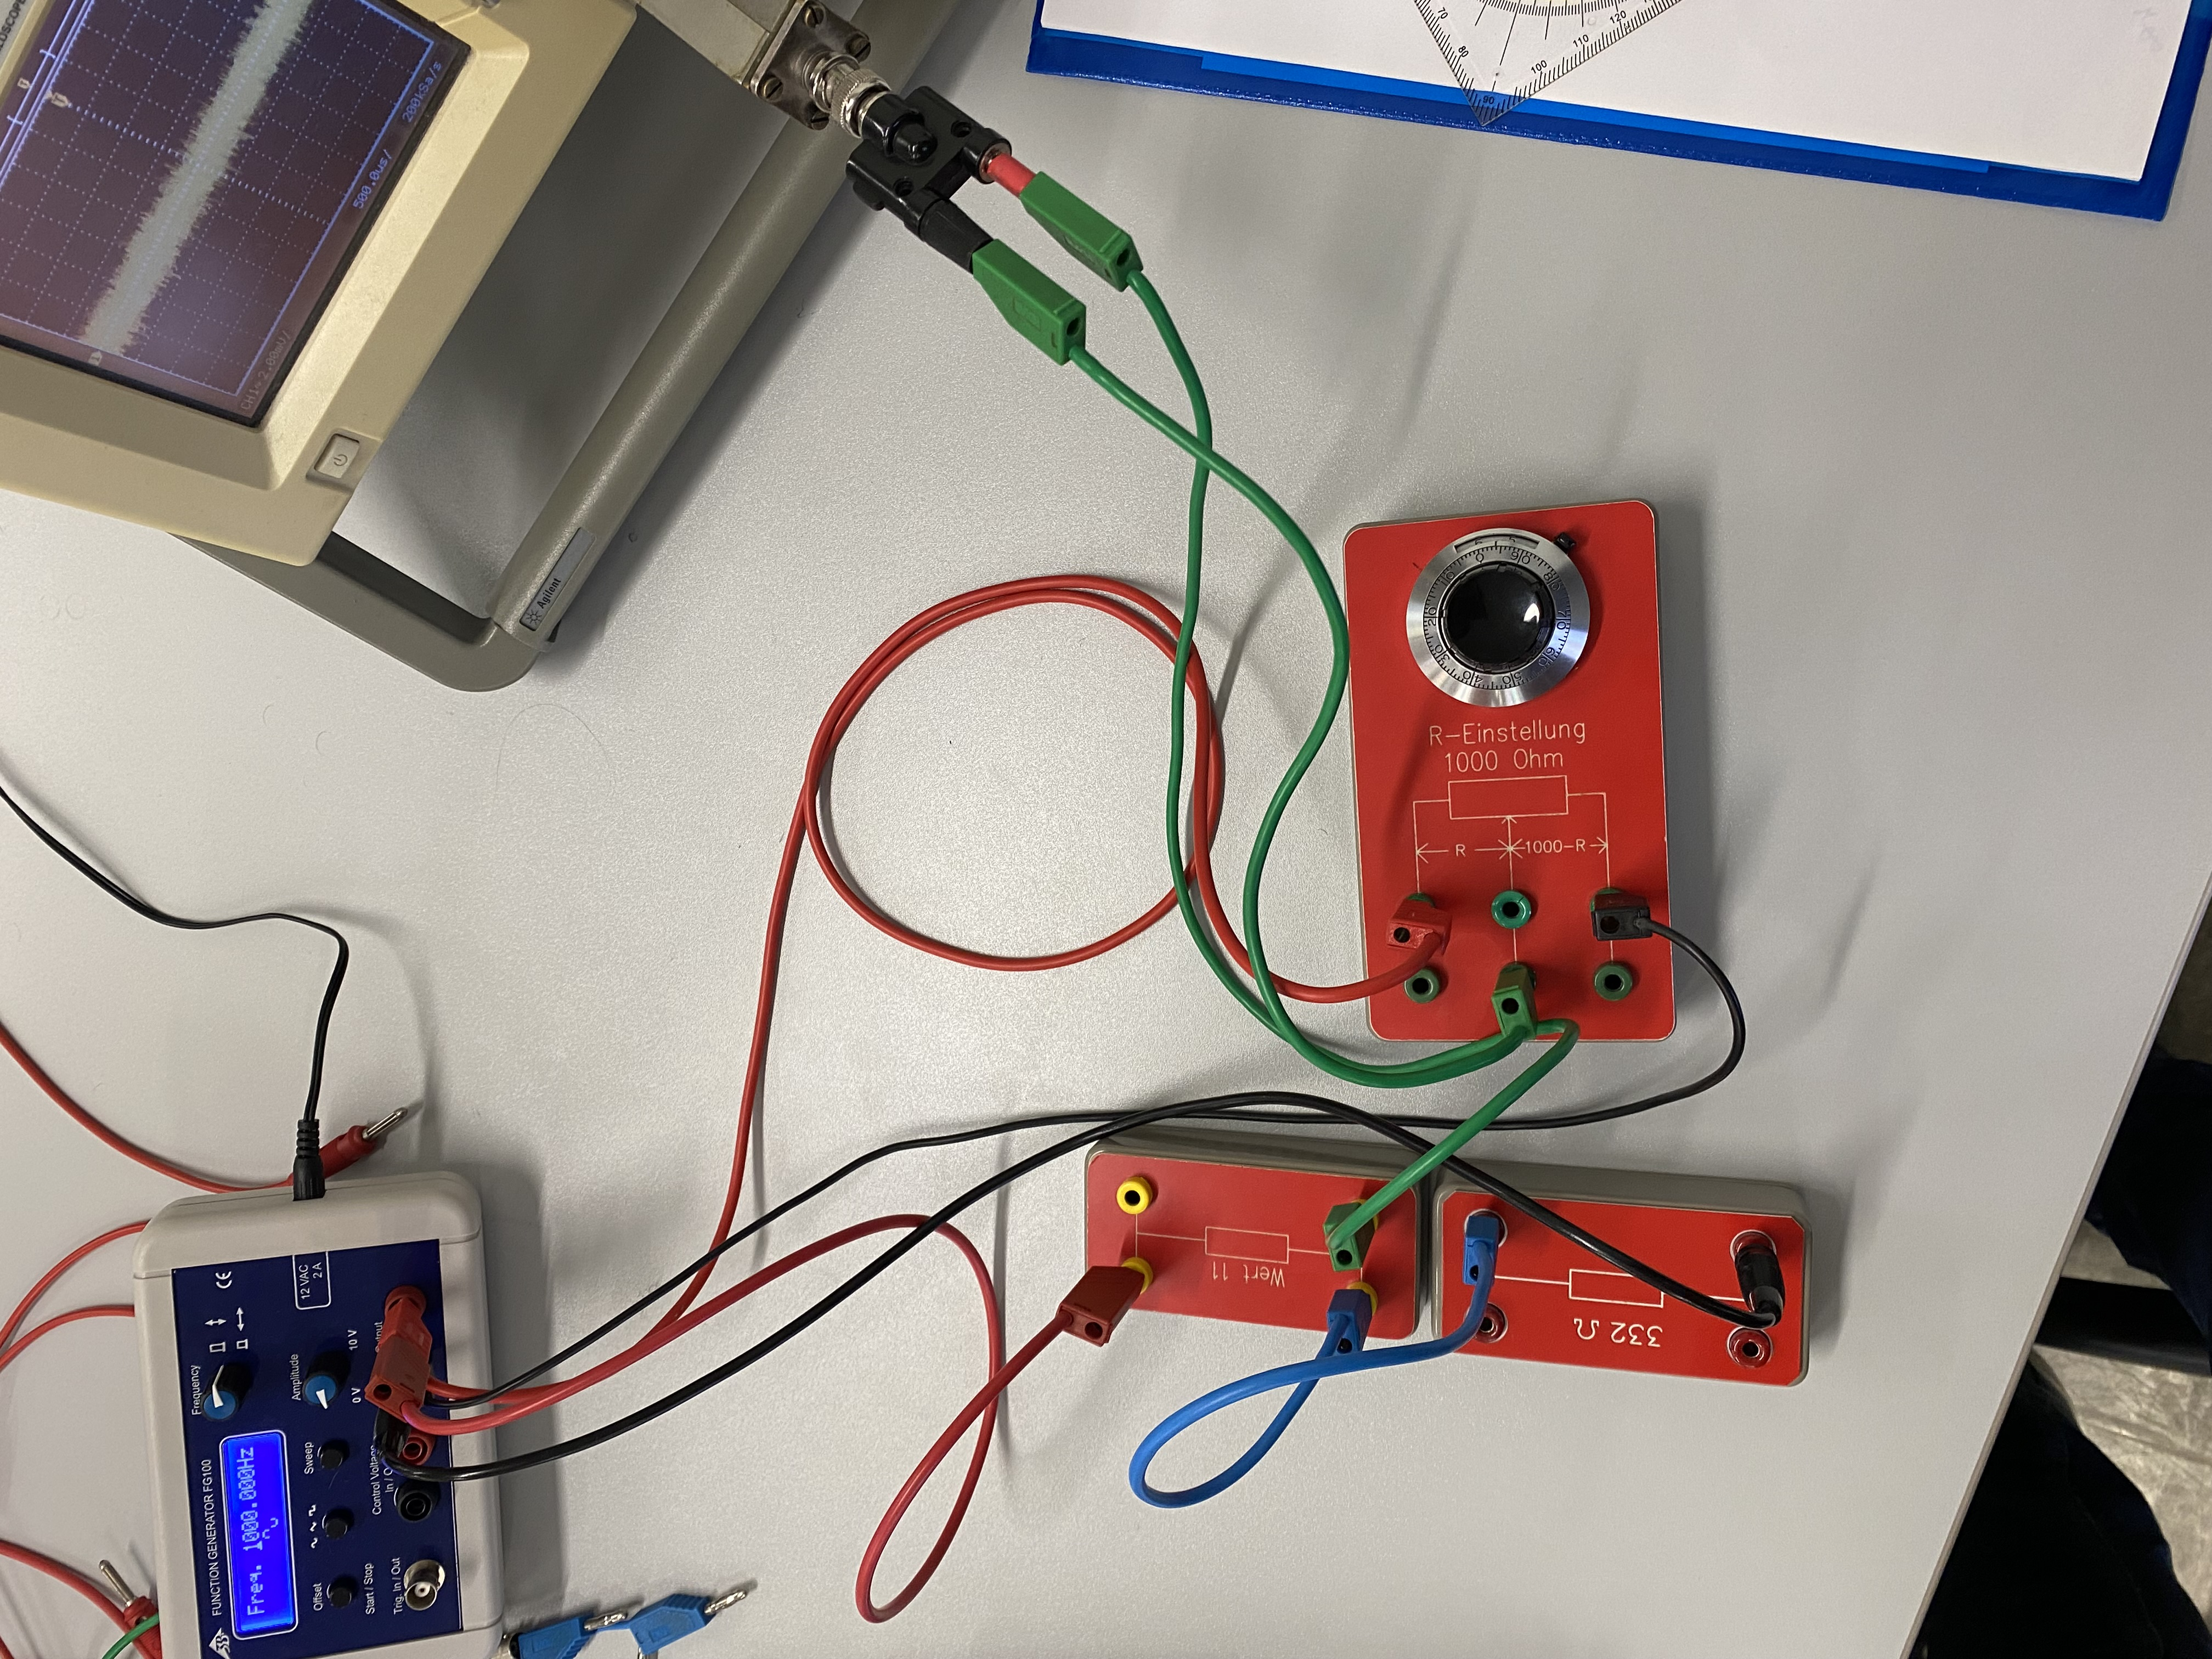
\includegraphics{Bilder/wheat.jpg}
    \caption{Die Wheatstonesche Brückenschaltung}
    \label{fig:wheat}
  \end{figure}
  \begin{figure}
    \centering
    \includegraphics{Bilder/kapazität.jpg}
    \caption{Die kapazitive Brückenschaltung}
    \label{fig:kapaz}
  \end{figure}
  \begin{figure}
    \centering
    \includegraphics{Bilder/induktivität.jpg}
    \caption{Die induktive Brückenschaltung}
    \label{fig:induk}
  \end{figure}
  \begin{figure}
    \centering
    \includegraphics{Bilder/maxwell.jpg}
    \caption{Die Maxwellsche Brückenschaltung}
    \label{fig:max}
  \end{figure}
  \begin{figure}
    \centering
    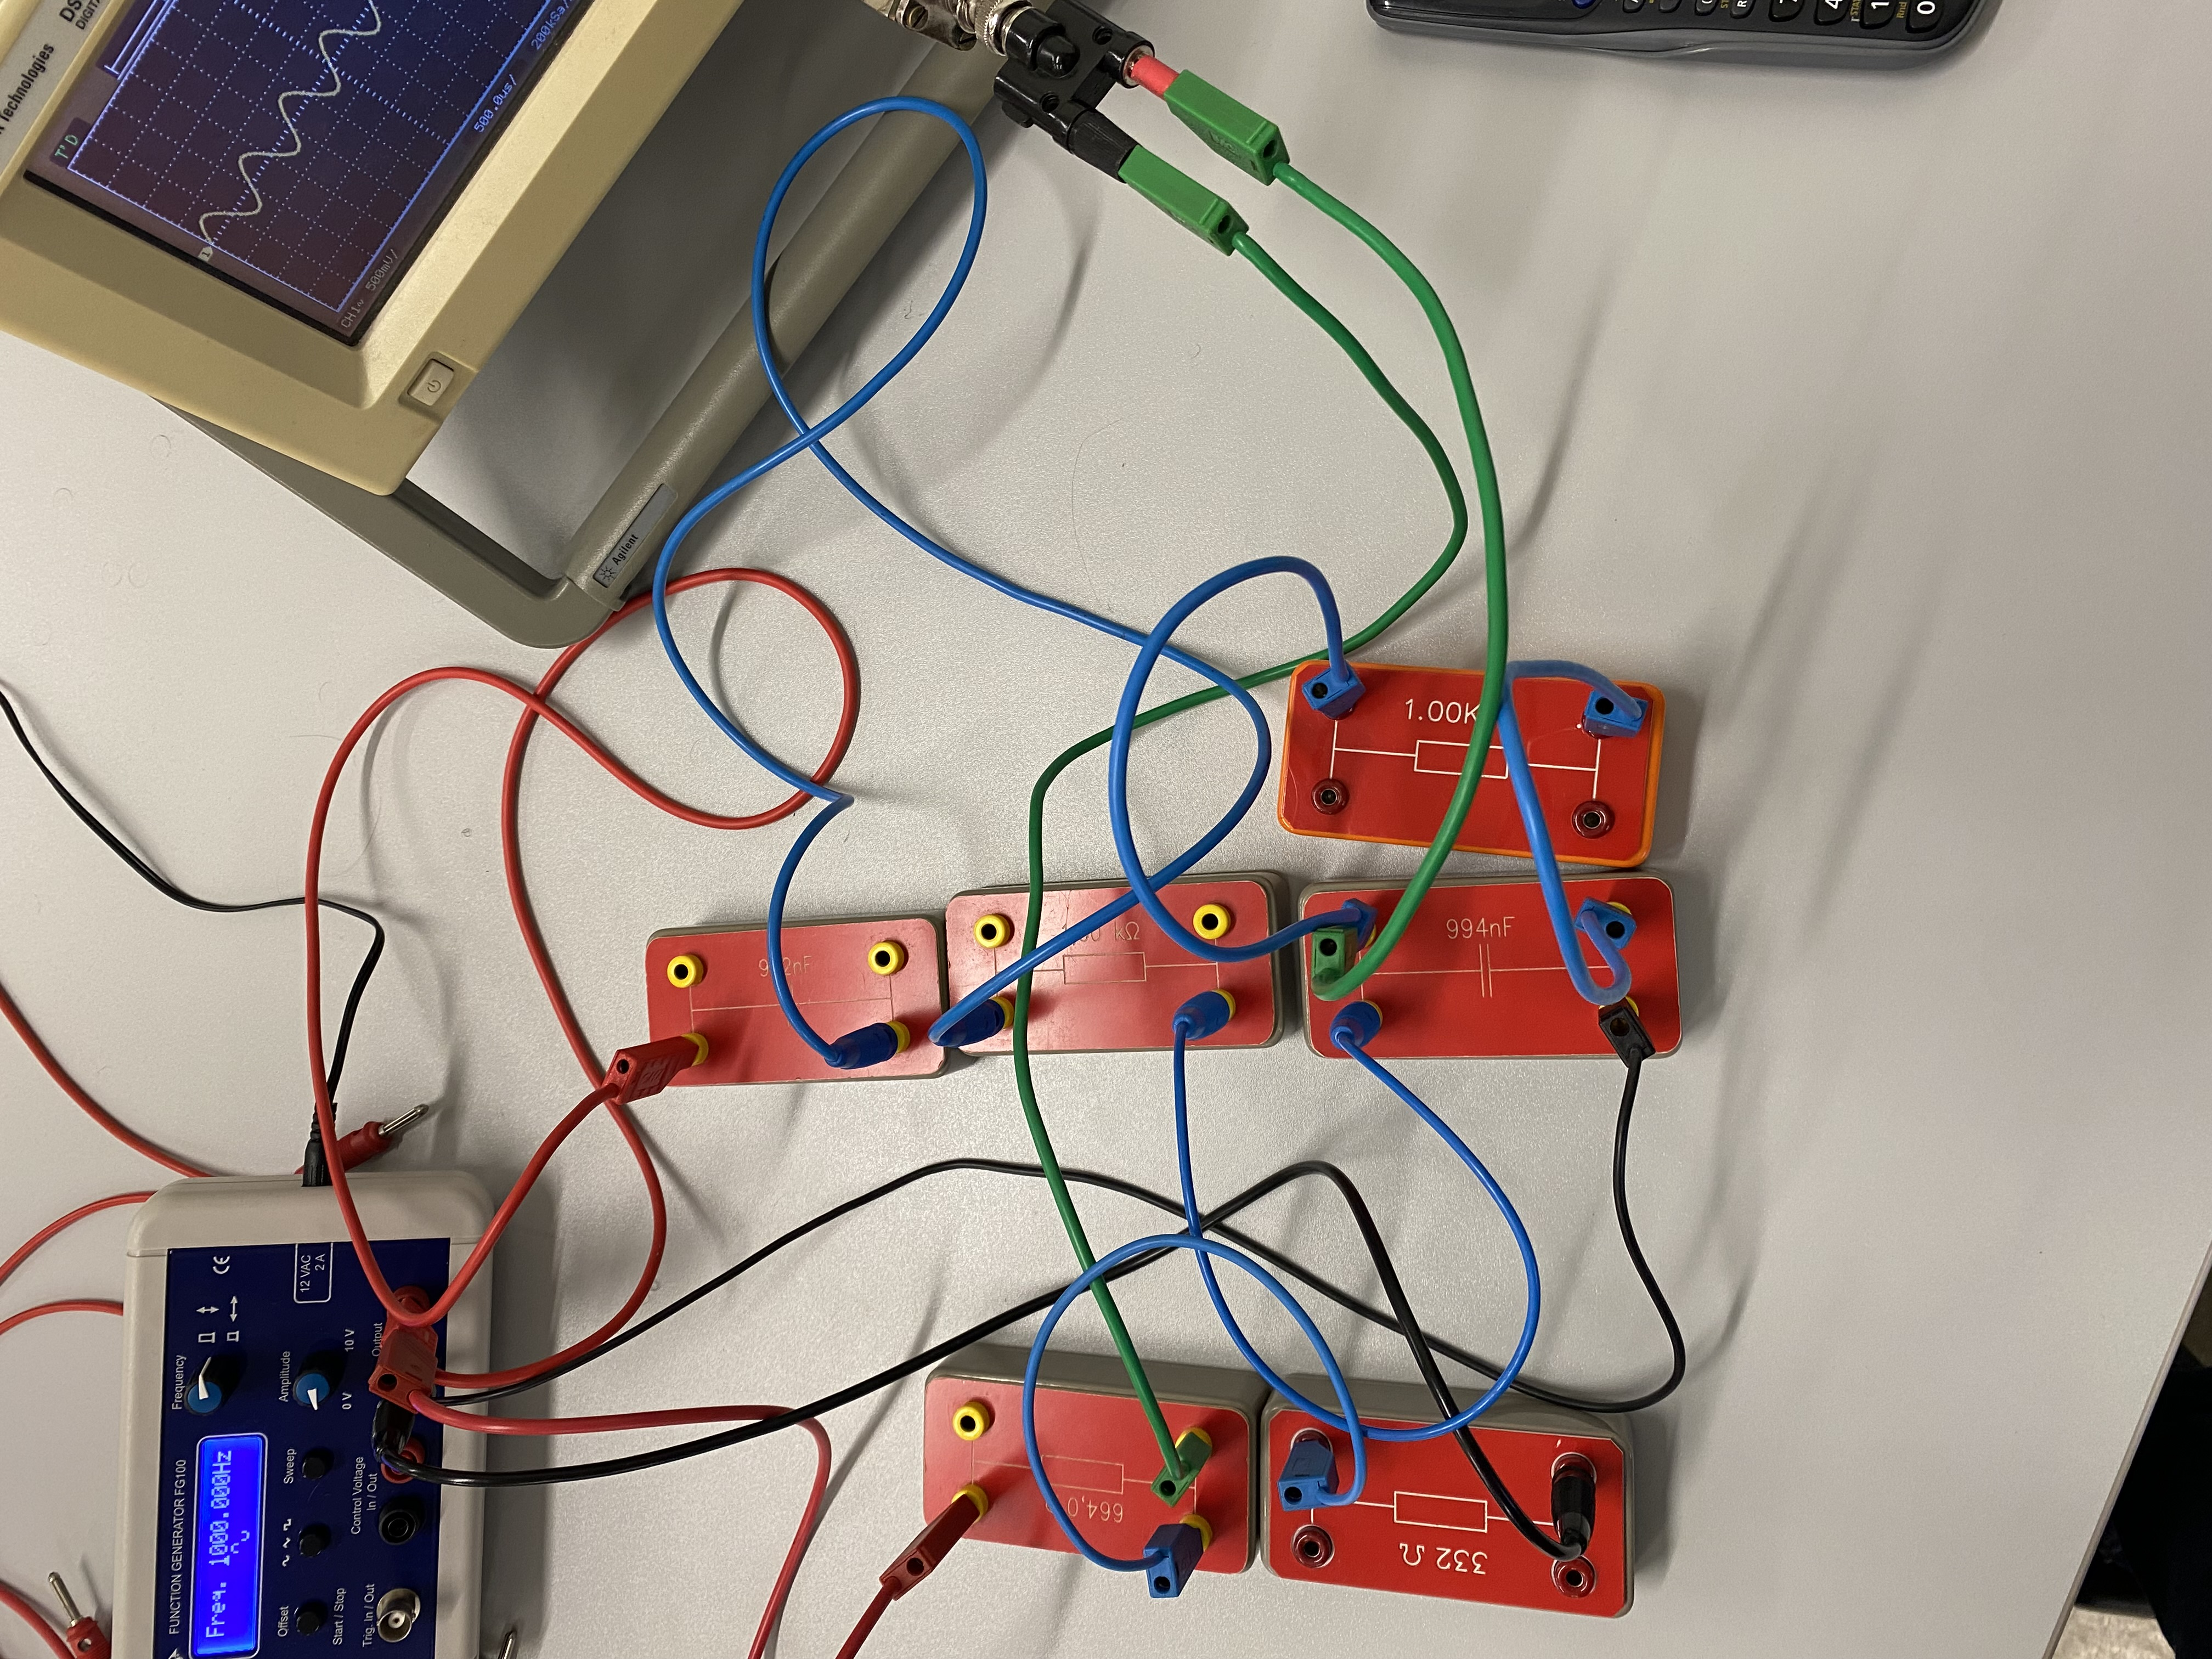
\includegraphics{Bilder/wien.jpg}
    \caption{Die Wien-Robinson Brückenschaltung}
    \label{fig:wheat}
  \end{figure}
  \begin{figure}
    \centering
    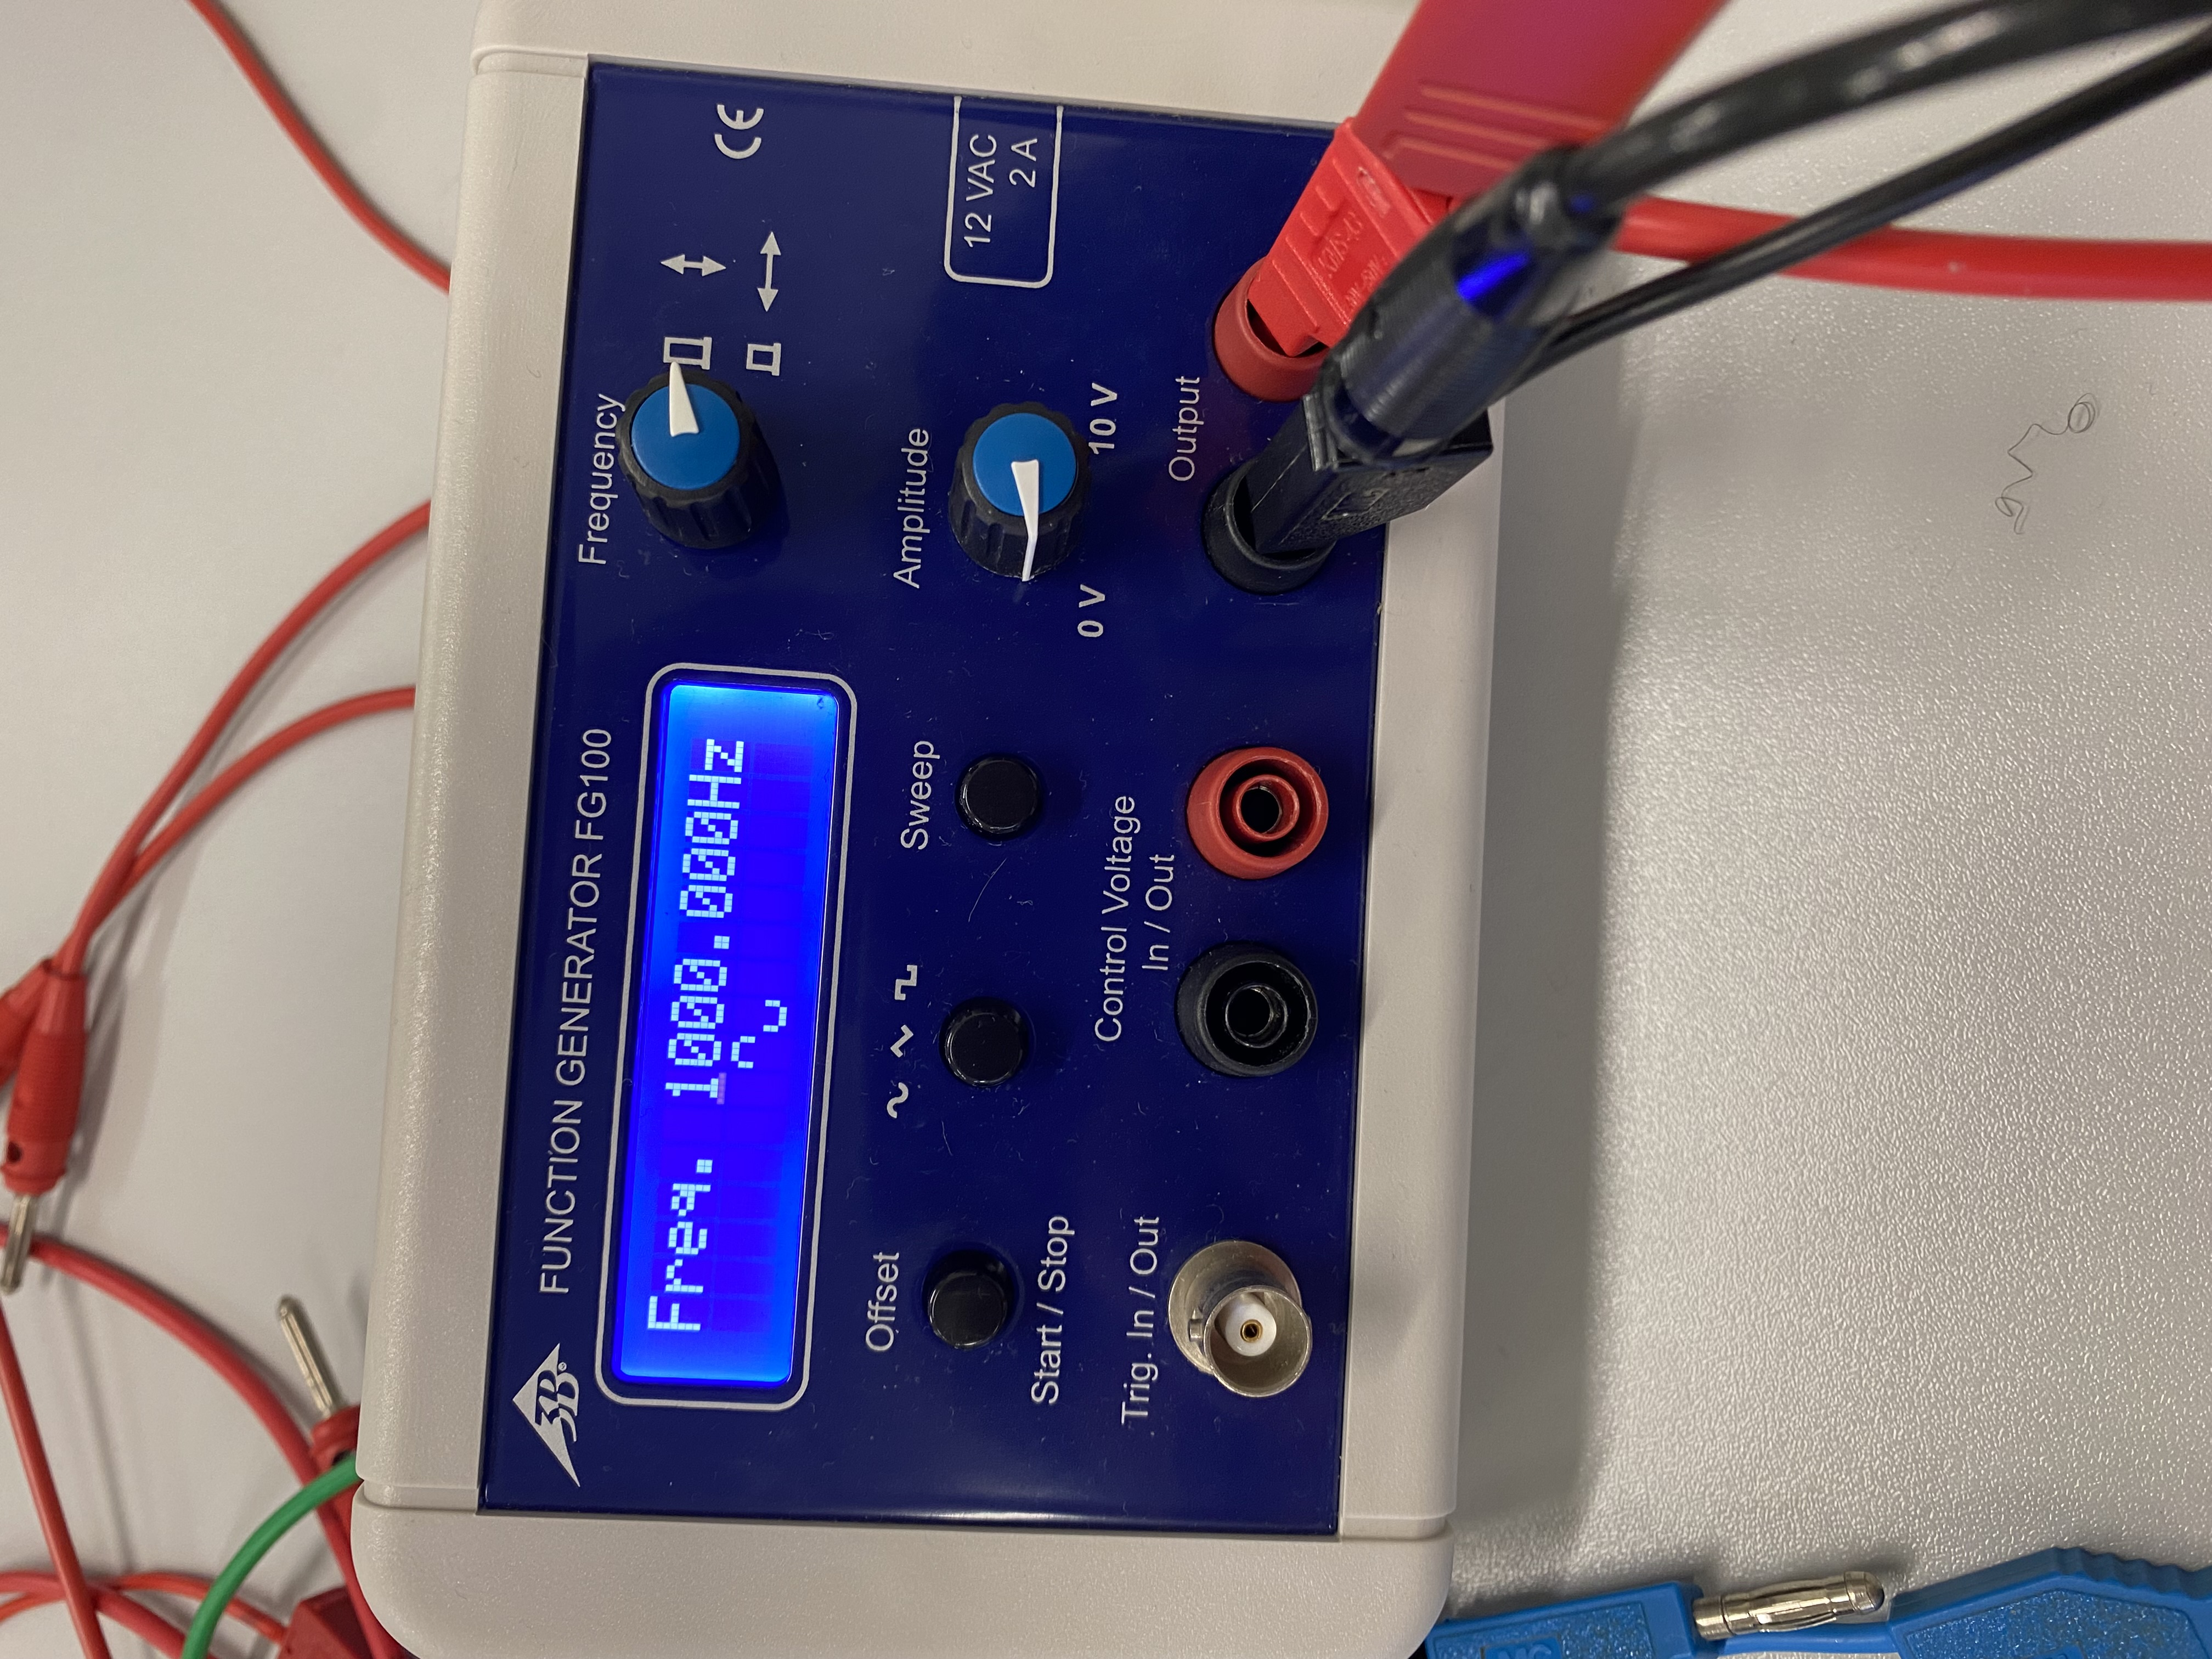
\includegraphics{Bilder/spannungsquelle.jpg}
    \caption{Die Wechselspannungsquelle}
    \label{fig:spann}
  \end{figure}
  \begin{figure}
    \centering
    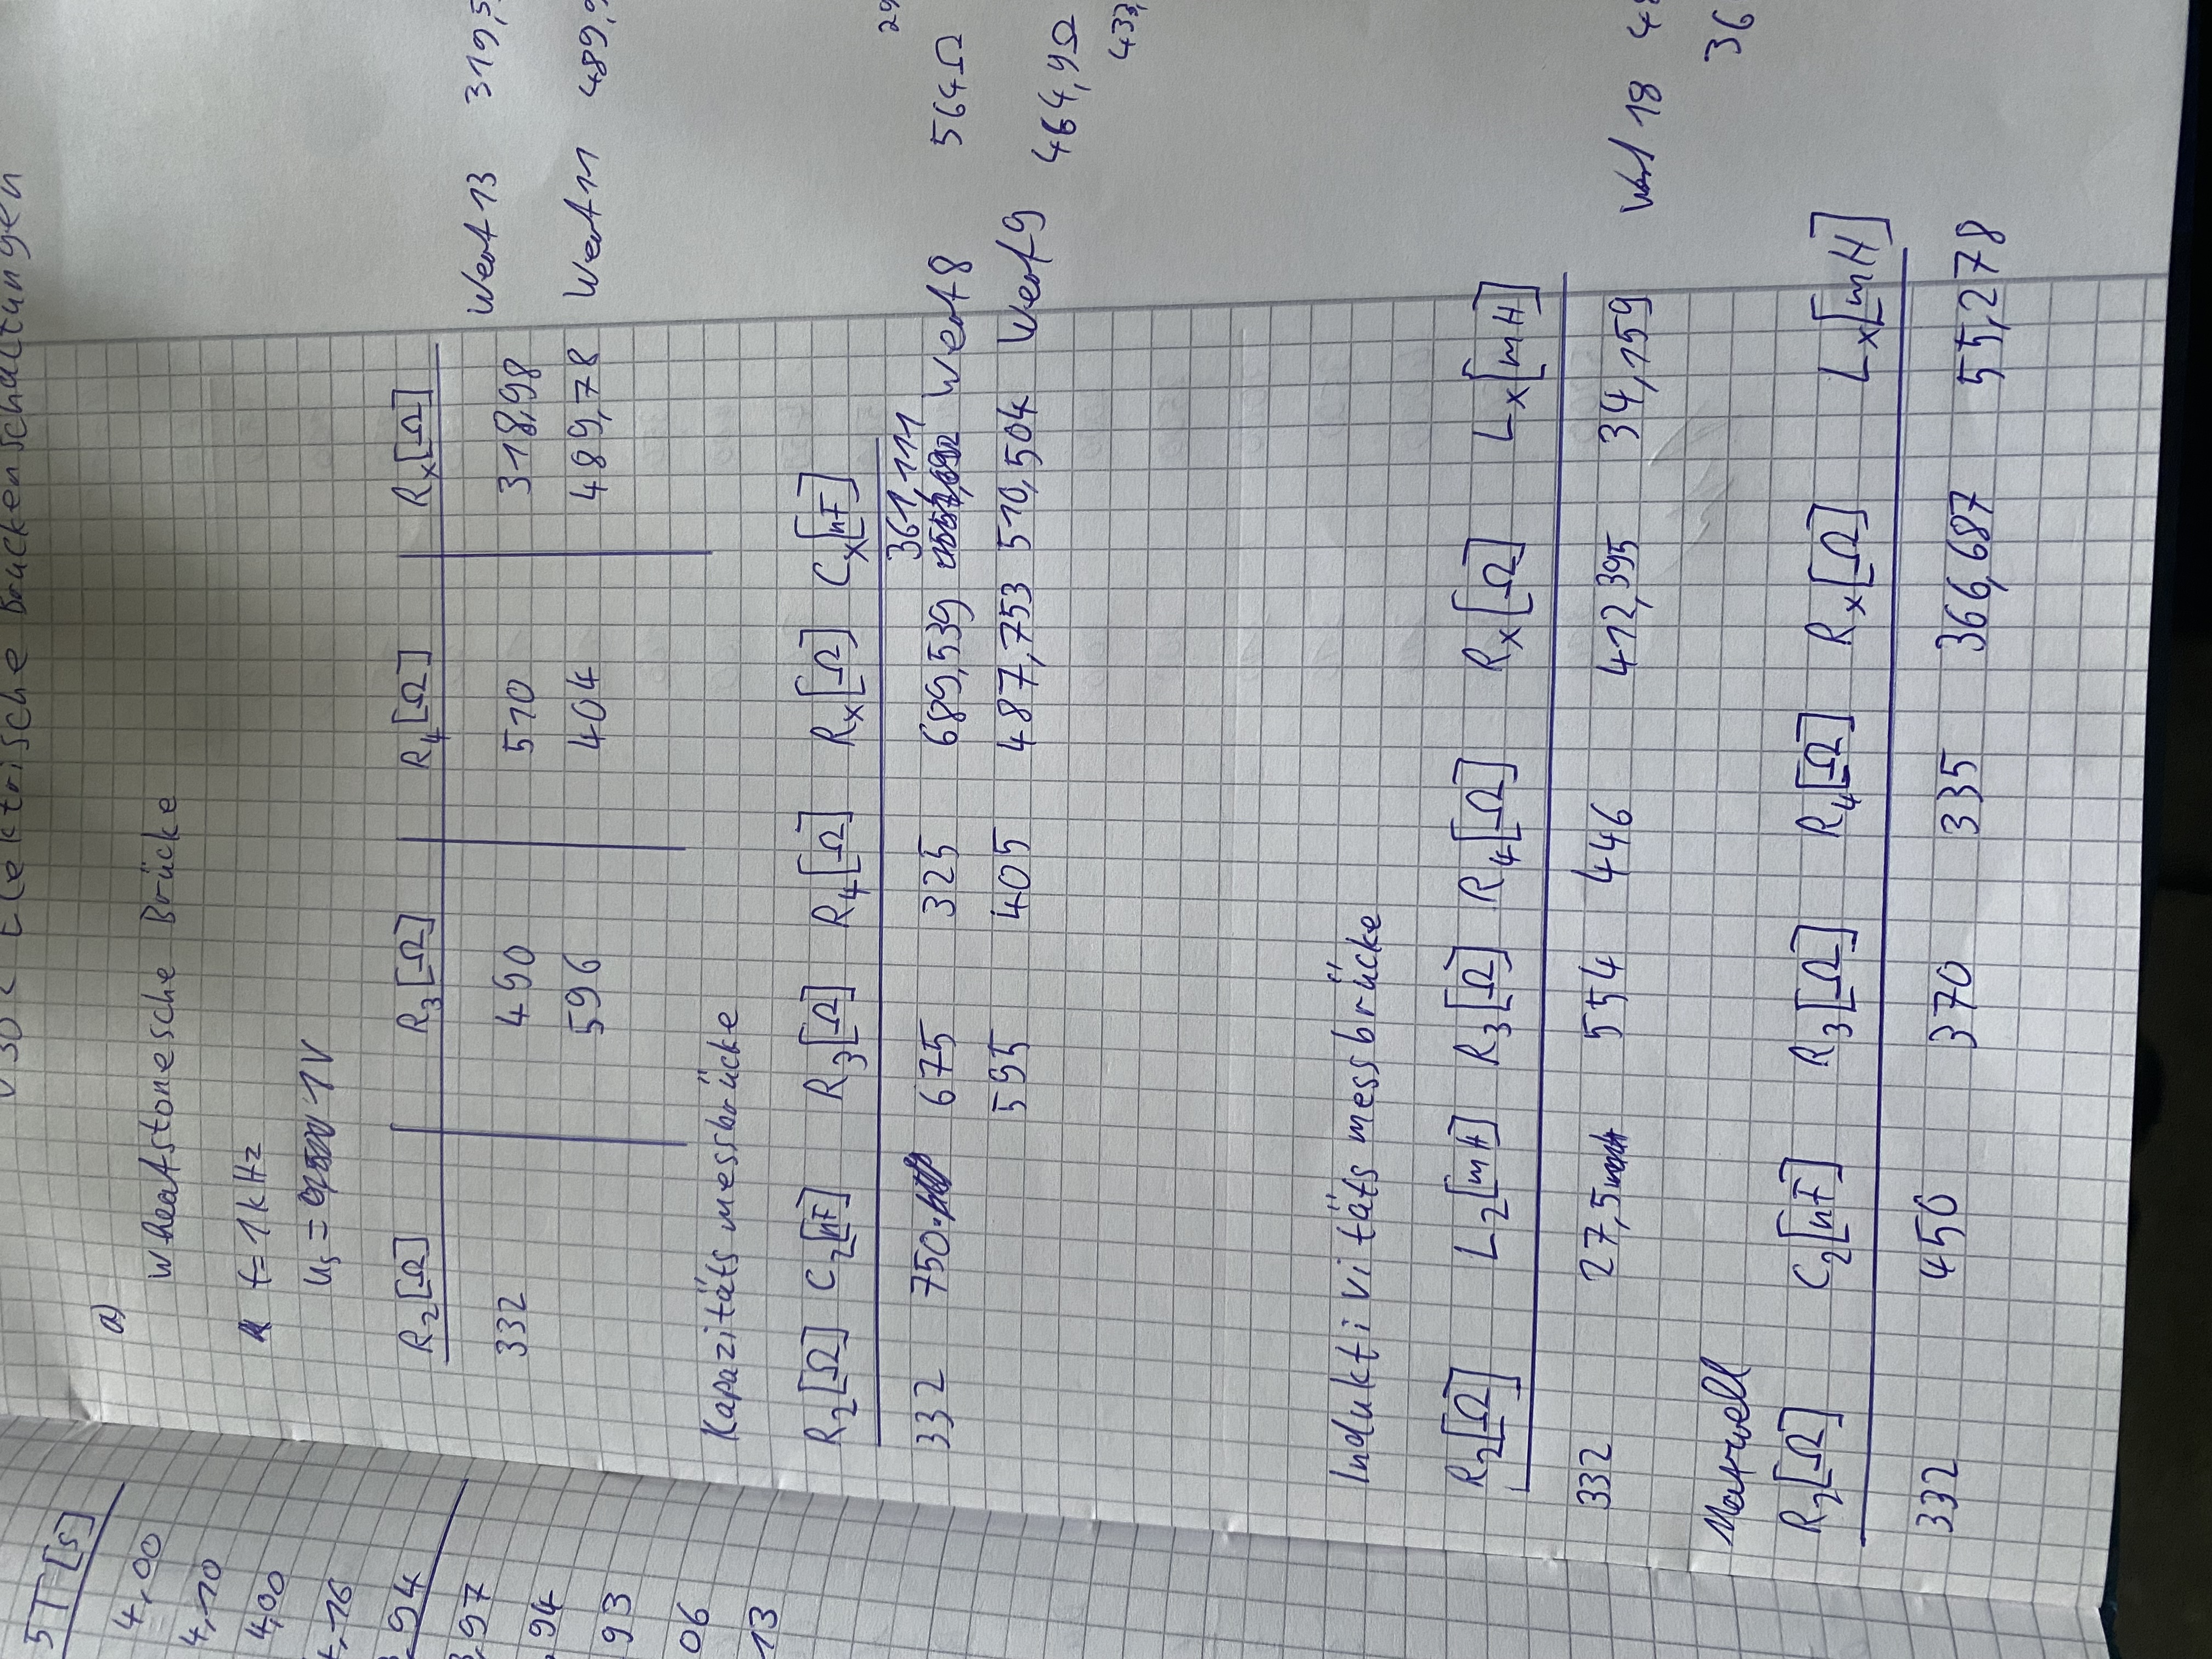
\includegraphics{Bilder/mess1.jpg}
    
    \label{fig:mess1}
  \end{figure}
  \begin{figure}
    \centering
    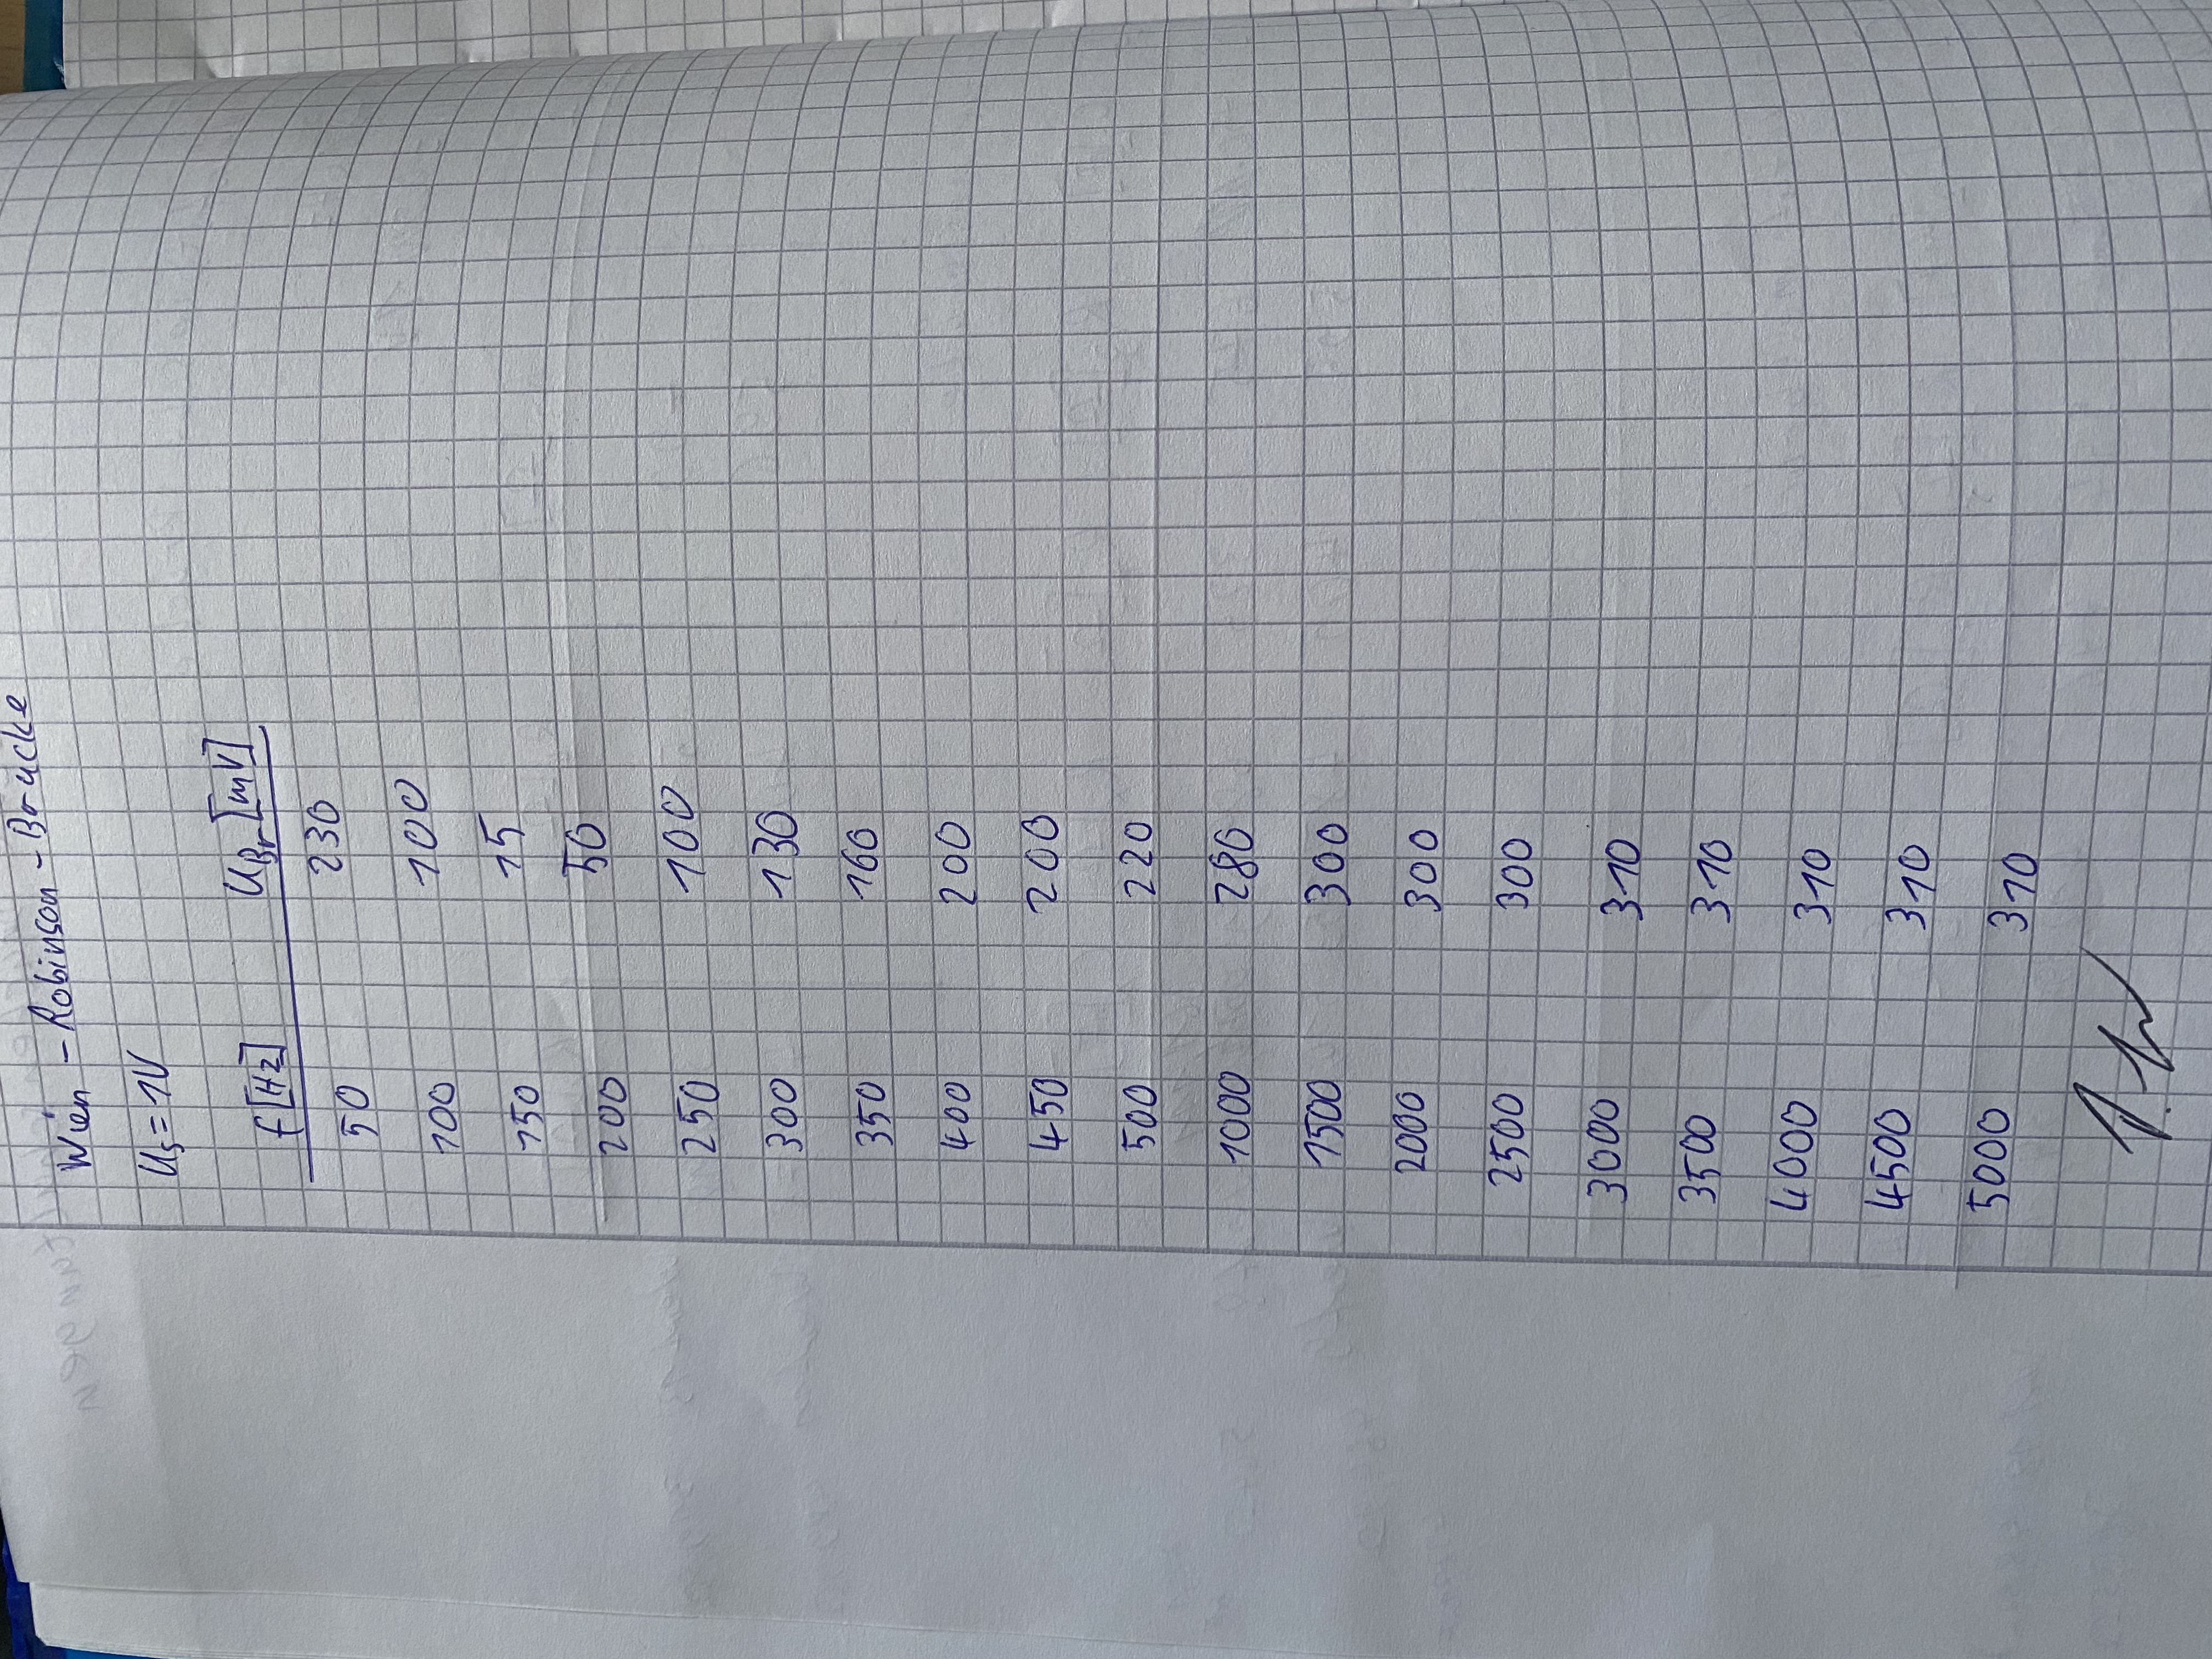
\includegraphics{Bilder/mess2.jpg}
  
    \label{fig:mess2}
  \end{figure}